\chapter{Risultati}
\label{cap:risultati}
In questo capitolo si presenta un'analisi dettagliata dei risultati ottenuti dagli esperimenti descritti in precedenza.
\section{Risultati degli Esperimenti CNN}
\subsection{Risultati Esperimento 1}
\subsubsection{Metriche di valutazione}
\begin{table}[ht]
    \centering
    \begin{tabular}{@{}|lcccc|@{}}
    \toprule
    \textbf{Classe}      & \textbf{Precision} & \textbf{Recall} & \textbf{F1-Score} & \textbf{Support} \\ \midrule
    Adware          & 0.84               & 0.85            & 0.85              & 446              \\
    Backdoor        & 0.90               & 0.45            & 0.60              & 135              \\
    Downloader      & 0.52               & 0.30            & 0.38              & 123              \\
    Ransomware      & 0.84               & 0.90            & 0.87              & 256              \\
    Spyware         & 0.00               & 0.00            & 0.00              & 43               \\
    Trojan          & 0.60               & 0.83            & 0.70              & 404              \\
    Virus           & 0.60               & 0.56            & 0.58              & 205              \\ \midrule
    \textbf{Accuracy}      & \multicolumn{3}{c}{\textbf{0.71}}         & 1612             \\ \midrule
    Macro Avg       & 0.61               & 0.56            & 0.57              & 1612             \\
    Weighted Avg    & 0.71               & 0.72            & 0.70              & 1612             \\ \bottomrule
    \end{tabular}
    \vspace{.2cm}
    \caption{\emph{Report di classificazione del modello CNN per la rilevazione di malware}}
    \label{tab:report_1_esperimento}
\end{table}
La tabella \ref{tab:report_1_esperimento} riassume le prestazioni del modello CNN per la classificazione delle diverse famiglie di malware, utilizzando metriche standard come precision, recall e F1-Score. I punti principali da evidenziare sono i seguenti:
\begin{itemize}
    \item \textbf{Adware:} Questa classe mostra ottime metriche, con valori di precision, recall e F1-Score pari a 0.85. Ciò indica che il modello è altamente efficace nel riconoscere i campioni di Adware.
    \item \textbf{Backdoor:} Sebbene la precision sia elevata (0.90), il recall è molto più basso (0.45), suggerendo che il modello non riesce a identificare una percentuale significativa di campioni di questa classe.
    \item \textbf{Downloader:} Le performance per questa classe sono scarse, con un F1-Score di 0.38, evidenziando problemi significativi nella corretta classificazione di questi campioni.
    \item \textbf{Spyware:} Questa classe presenta le peggiori performance, con un F1-Score di 0.00, indicando che il modello non è in grado di riconoscere alcun campione di Spyware.
    \item \textbf{Ransomware:} Il modello mostra buone prestazioni su questa classe, con un F1-Score di 0.87, grazie a valori bilanciati di precision (0.84) e recall (0.90).
    \item \textbf{Trojan:} La precision è moderata (0.60), ma il recall elevato (0.83) porta a un F1-Score di 0.70. Questo suggerisce che il modello riconosce correttamente molti campioni di Trojan, ma a costo di alcune classificazioni errate.
    \item \textbf{Virus:} Con un F1-Score di 0.58, questa classe presenta una moderata confusione rispetto ad altre categorie.
\end{itemize}
Globalmente, l'accuracy del modello è pari a 72\%, ma le metriche di \textit{macro average} (0.57 per F1-Score) evidenziano come il modello non gestisca uniformemente tutte le classi, con significative difficoltà per le classi meno rappresentate come Spyware e Downloader.
\subsubsection{Matrice di Confusione}
\begin{table}[ht]
    \centering
    \hspace*{-2cm} 
    \begin{tabular}{@{}|l|c|c|c|c|c|c|c|@{}}
    \toprule
    \textbf{Classe}      & \textbf{Adware} & \textbf{Backdoor} & \textbf{Downloader} & \textbf{Ransomware} & \textbf{Spyware} & \textbf{Trojan} & \textbf{Virus} \\ \midrule
    \textbf{Adware}      & 380 & 0   & 2   & 0   & 0   & 31  & 33  \\\midrule
    \textbf{Backdoor}    & 3   & 61  & 12  & 15  & 0   & 39  & 5   \\\midrule
    \textbf{Downloader}  & 8   & 3   & 37  & 1   & 0   & 65  & 9   \\\midrule
    \textbf{Ransomware}  & 0   & 0   & 1   & 230 & 0   & 16  & 9   \\\midrule
    \textbf{Spyware}     & 0   & 1   & 6   & 3   & 0   & 30  & 3   \\\midrule
    \textbf{Trojan}      & 17  & 2   & 9   & 26  & 0   & 334 & 16  \\\midrule
    \textbf{Virus}       & 44  & 1   & 4   & 0   & 0   & 42  & 114 \\ \bottomrule
    \end{tabular}
    \vspace{.2cm}
    \caption{\emph{Matrice di Confusione: confronto tra classi reali (righe) e classi predette (colonne)}}
    \label{tab:confusion_matrix_1_esperimento}
\end{table}
La matrice di confusione presentata in Tabella \ref{tab:confusion_matrix_1_esperimento} offre una visione dettagliata delle predizioni del modello, evidenziando le aree di forza e le principali difficoltà nella classificazione delle famiglie di malware:
\begin{itemize}
    \item \textbf{Adware:} Questa classe è ben classificata, con 380 predizioni corrette su 446. Tuttavia, alcune istanze sono confuse con Trojan (31) e Virus (33), suggerendo una certa sovrapposizione nelle caratteristiche di queste classi.
    \item \textbf{Backdoor:} Solo 61 campioni su 135 sono classificati correttamente. Molti errori coinvolgono Trojan (39) e Downloader (12), evidenziando che queste classi presentano pattern simili.
    \item \textbf{Downloader:} La performance per questa classe è particolarmente scarsa, con solo 37 predizioni corrette su 123. La maggior parte degli errori si verifica verso Trojan (65), indicando che il modello non riesce a distinguere efficacemente tra queste due categorie.
    \item \textbf{Ransomware:} Questa è una delle classi meglio classificate, con 230 predizioni corrette su 256. Gli errori principali si distribuiscono tra Trojan (16) e Virus (9), ma in generale il modello gestisce bene questa classe.
    \item \textbf{Spyware:} Nonostante abbia solo 43 campioni, il modello non riesce a classificare correttamente alcuna istanza. Gli errori principali coinvolgono Trojan (30), suggerendo una sovrapposizione significativa nelle caratteristiche.
    \item \textbf{Trojan:} Con 334 predizioni corrette su 404, il modello gestisce bene questa classe. Tuttavia, vi è confusione con Adware (17) e Downloader (9), evidenziando la necessità di migliorare il modello per separare meglio queste categorie.
    \item \textbf{Virus:} Con 114 predizioni corrette su 205, la classe Virus presenta errori significativi, principalmente verso Trojan (42) e Adware (44). Questo suggerisce che il modello fatica a distinguere tra Virus e altre classi con pattern simili.
\end{itemize}
In generale, la matrice di confusione mostra che il modello funziona bene per classi come Adware e Ransomware, ma ha difficoltà significative con le classi Spyware, Downloader e Backdoor. Questi risultati evidenziano la necessità di ulteriori ottimizzazioni per migliorare la discriminazione tra classi con pattern sovrapposti e rafforzare la gestione delle classi meno rappresentate.


\subsection{Risultati Esperimento 2}
\subsubsection{Metriche di valutazione}
\begin{table}[ht]
    \centering
    \begin{tabular}{@{}|lcccc|@{}}
    \toprule
    \textbf{Classe}      & \textbf{Precision} & \textbf{Recall} & \textbf{F1-Score} & \textbf{Support} \\ \midrule
    Adware          & 0.87               & 0.91            & 0.89              & 446              \\
    Backdoor        & 0.87               & 0.72            & 0.79              & 135              \\
    Downloader      & 0.71               & 0.61            & 0.66              & 123              \\
    Ransomware      & 0.86               & 0.94            & 0.90              & 256              \\
    Spyware         & 0.59               & 0.51            & 0.55              & 43               \\
    Trojan          & 0.77               & 0.79            & 0.78              & 404              \\
    Virus           & 0.73               & 0.68            & 0.70              & 205              \\ \midrule
    \textbf{Accuracy}      & \multicolumn{3}{c}{\textbf{0.81}}         & 1612             \\ \midrule
    Macro Avg       & 0.77               & 0.74            & 0.75              & 1612             \\
    Weighted Avg    & 0.80               & 0.81            & 0.80              & 1612             \\ \bottomrule
    \end{tabular}
    \vspace{.2cm}
    \caption{\emph{Report di classificazione del modello CNN per la rilevazione di malware}}
    \label{tab:report_2_esperimento}
\end{table}
La tabella \ref{tab:report_2_esperimento} riassume le prestazioni del modello CNN per la classificazione delle diverse famiglie di malware, utilizzando metriche standard come precision, recall e F1-Score. I punti principali da evidenziare sono i seguenti:
\begin{itemize}
    \item \textbf{Adware:} Questa classe mostra prestazioni eccellenti, con valori di precision, recall e F1-Score pari a 0.87, 0.91 e 0.89 rispettivamente. Ciò indica che il modello è molto efficace nel riconoscere i campioni di Adware.
    \item \textbf{Backdoor:} Nonostante una precision alta (0.87), il recall è inferiore (0.72), evidenziando difficoltà del modello nel riconoscere tutti i campioni di Backdoor.
    \item \textbf{Downloader:} Questa classe presenta prestazioni moderate, con un F1-Score di 0.66. La precision (0.71) e il recall (0.61) suggeriscono che il modello ha problemi a distinguere Downloader da altre classi.
    \item \textbf{Spyware:} Mostra performance deboli, con un F1-Score di 0.55. Sebbene la precision sia accettabile (0.59), il basso recall (0.51) indica che molti campioni di Spyware non vengono correttamente identificati.
    \item \textbf{Ransomware:} Questa classe è una delle meglio riconosciute dal modello, con un F1-Score di 0.90 e recall molto alto (0.94).
    \item \textbf{Trojan:} La precision (0.77) e il recall (0.79) portano a un F1-Score di 0.78. Ciò suggerisce una buona capacità del modello nel classificare questa classe.
    \item \textbf{Virus:} Con un F1-Score di 0.70, questa classe è moderatamente ben gestita, ma i valori di precision e recall (0.73 e 0.68) indicano ancora una certa confusione con altre classi.
\end{itemize}
L'accuracy complessiva è pari a 80.71\%, indicando buone prestazioni globali del modello. Tuttavia, le metriche \textit{macro average} (0.75 per F1-Score) evidenziano che alcune classi meno rappresentate, come Spyware, richiedono ulteriori ottimizzazioni.
\subsubsection{Matrice di Confusione}
\begin{table}[ht]
    \centering
    \hspace*{-2cm} 
    \begin{tabular}{@{}|l|c|c|c|c|c|c|c|@{}}
    \toprule
    \textbf{Classe}      & \textbf{Adware} & \textbf{Backdoor} & \textbf{Downloader} & \textbf{Ransomware} & \textbf{Spyware} & \textbf{Trojan} & \textbf{Virus} \\ \midrule
    \textbf{Adware}      & 407 & 0   & 5   & 1   & 3   & 15  & 15  \\\midrule
    \textbf{Backdoor}    & 7   & 97  & 1   & 4   & 1   & 18  & 7   \\\midrule
    \textbf{Downloader}  & 5   & 2   & 75  & 5   & 2   & 26  & 8   \\\midrule
    \textbf{Ransomware}  & 0   & 0   & 5   & 240 & 1   & 10  & 0   \\\midrule
    \textbf{Spyware}     & 1   & 2   & 4   & 2   & 22  & 10  & 2   \\\midrule
    \textbf{Trojan}      & 16  & 7   & 10  & 23  & 7   & 320 & 21  \\\midrule
    \textbf{Virus}       & 34  & 3   & 5   & 5   & 1   & 17  & 140 \\ \bottomrule
    \end{tabular}
    \vspace{.2cm}
    \caption{\emph{Matrice di Confusione: confronto tra classi reali (righe) e classi predette (colonne)}}
    \label{tab:confusion_matrix_2_esperimento}
\end{table}
La matrice di confusione riportata in Tabella \ref{tab:confusion_matrix_2_esperimento} evidenzia le seguenti osservazioni:
\begin{itemize}
    \item \textbf{Adware:} Con 407 predizioni corrette su 446, questa classe è ben classificata. Tuttavia, alcune istanze vengono confuse principalmente con Trojan (15) e Virus (15).
    \item \textbf{Backdoor:} Ha 97 predizioni corrette su 135. Gli errori principali coinvolgono Trojan (18) e Adware (7), suggerendo che queste classi presentano caratteristiche sovrapposte.
    \item \textbf{Downloader:} Mostra 75 predizioni corrette su 123, con errori significativi verso Trojan (26) e Virus (8), indicando difficoltà del modello nel distinguere tra queste categorie.
    \item \textbf{Ransomware:} Questa classe è ben riconosciuta, con 240 predizioni corrette su 256. Gli errori principali si distribuiscono tra Trojan (10) e Virus (5).
    \item \textbf{Spyware:} Con solo 22 predizioni corrette su 43, il modello confonde spesso questa classe con Trojan (10) e Adware (1), evidenziando una scarsa capacità di discriminazione.
    \item \textbf{Trojan:} È una delle classi più rappresentate, con 320 predizioni corrette su 404. Tuttavia, vi è una confusione moderata con Adware (16) e Downloader (10).
    \item \textbf{Virus:} Ha 140 predizioni corrette su 205. Gli errori principali coinvolgono Trojan (17) e Adware (34), suggerendo difficoltà nel distinguere Virus da altre classi con pattern simili.
\end{itemize}
La matrice di confusione evidenzia che, sebbene il modello funzioni bene per classi come Adware e Ransomware, presenta difficoltà significative nel distinguere classi meno rappresentate o con caratteristiche sovrapposte, come Spyware e Downloader.


\subsection{Risultati Esperimento 3}
Grazie alla configurabilità dinamica degli iperparametri e al processo di tuning, questo approccio consente di adattare il modello alle specifiche del dataset e di massimizzarne le prestazioni nella classificazione dei malware.
\subsubsection{Metriche di valutazione}
\begin{table}[ht]
    \centering
    \begin{tabular}{@{}|lcccc|@{}}
    \toprule
    \textbf{Classe}      & \textbf{Precision} & \textbf{Recall} & \textbf{F1-Score} & \textbf{Support} \\ \midrule
    Adware          & 0.87               & 0.93            & 0.90              & 446              \\
    Backdoor        & 0.81               & 0.78            & 0.80              & 135              \\
    Downloader      & 0.78               & 0.56            & 0.65              & 123              \\
    Ransomware      & 0.85               & 0.95            & 0.89              & 256              \\
    Spyware         & 0.66               & 0.49            & 0.56              & 43               \\
    Trojan          & 0.76               & 0.82            & 0.79              & 404              \\
    Virus           & 0.81               & 0.65            & 0.72              & 205              \\ \midrule
    \textbf{Accuracy}      & \multicolumn{3}{c}{\textbf{0.82}}         & 1612             \\ \midrule
    Macro Avg       & 0.79               & 0.74            & 0.76              & 1612             \\
    Weighted Avg    & 0.81               & 0.82            & 0.81              & 1612             \\ \bottomrule
    \end{tabular}
    \vspace{.2cm}
    \caption{\emph{Report di classificazione del modello CNN per la rilevazione di malware}}
    \label{tab:report_3_esperimento}
\end{table}
La Tabella \ref{tab:report_3_esperimento} presenta le metriche di classificazione del modello CNN per ciascuna delle classi di malware. Di seguito sono evidenziati i principali risultati:
\begin{itemize}
    \item \textbf{Adware:} Questa classe raggiunge le migliori prestazioni complessive, con precision, recall e F1-Score molto elevati (rispettivamente 0.87, 0.93 e 0.90). Ciò indica che il modello identifica correttamente la maggior parte dei campioni di Adware, con pochi falsi positivi e falsi negativi.
    
    \item \textbf{Backdoor:} Con un F1-Score di 0.80, il modello mostra una buona capacità di classificare i campioni di Backdoor. Tuttavia, la precision (0.81) e il recall (0.78) evidenziano una certa confusione rispetto ad altre classi.
    
    \item \textbf{Downloader:} Le prestazioni per questa classe sono moderate, con un F1-Score di 0.65. Il recall più basso (0.56) suggerisce che il modello non riesce a riconoscere una porzione significativa di campioni di Downloader, anche se la precision (0.78) indica che i campioni classificati come Downloader sono in gran parte corretti.
    
    \item \textbf{Ransomware:} Questa classe è una delle meglio gestite dal modello, con un F1-Score di 0.89 e un recall molto alto (0.95), dimostrando che il modello identifica correttamente quasi tutti i campioni di Ransomware.
    
    \item \textbf{Spyware:} Le prestazioni per questa classe sono significativamente inferiori rispetto alle altre, con un F1-Score di 0.56 e un recall particolarmente basso (0.49). Ciò suggerisce difficoltà significative nel distinguere i campioni di Spyware da quelli di altre classi.
    
    \item \textbf{Trojan:} Con un F1-Score di 0.79, il modello dimostra una buona capacità di identificare i Trojan. Il recall (0.82) indica che molti campioni di questa classe vengono correttamente riconosciuti, sebbene vi siano alcune confusioni con altre categorie.
    
    \item \textbf{Virus:} Le prestazioni per questa classe sono moderate, con un F1-Score di 0.72. Il recall più basso (0.65) suggerisce che alcuni campioni di Virus non vengono identificati correttamente.
\end{itemize}
L'accuracy globale del modello è del 82\%, indicando buone prestazioni complessive. Tuttavia, le metriche \textit{Macro Avg} (F1-Score di 0.76) e \textit{Weighted Avg} (F1-Score di 0.81) riflettono una distribuzione non uniforme delle prestazioni tra le diverse classi, con Spyware e Downloader che rappresentano i maggiori punti critici.
\subsubsection{Matrice di Confusione}
\begin{table}[ht]
    \centering
    \hspace*{-2cm} 
    \begin{tabular}{@{}|l|c|c|c|c|c|c|c|@{}}
    \toprule
    \textbf{Classe}      & \textbf{Adware} & \textbf{Backdoor} & \textbf{Downloader} & \textbf{Ransomware} & \textbf{Spyware} & \textbf{Trojan} & \textbf{Virus} \\ \midrule
    \textbf{Adware}      & 415 & 1   & 3   & 0   & 2   & 15  & 10  \\\midrule
    \textbf{Backdoor}    & 4   & 105 & 2   & 3   & 1   & 20  & 0   \\\midrule
    \textbf{Downloader}  & 7   & 10  & 69  & 6   & 1   & 27  & 3   \\\midrule
    \textbf{Ransomware}  & 0   & 0   & 3   & 242 & 1   & 10  & 0   \\\midrule
    \textbf{Spyware}     & 1   & 1   & 3   & 3   & 21  & 14  & 0   \\\midrule
    \textbf{Trojan}      & 13  & 8   & 5   & 25  & 4   & 331 & 18  \\\midrule
    \textbf{Virus}       & 38  & 4   & 4   & 7   & 2   & 17  & 133 \\ \bottomrule
    \end{tabular}
    \vspace{.2cm}
    \caption{\emph{Matrice di Confusione: confronto tra classi reali (righe) e classi predette (colonne)}}
    \label{tab:confusion_matrix_3_esperimento}
\end{table}
La matrice di confusione riportata in Tabella \ref{tab:confusion_matrix_3_esperimento} fornisce una visione dettagliata delle predizioni del modello, evidenziando le aree di forza e le principali difficoltà:
\begin{itemize}
    \item \textbf{Adware:} Con 415 predizioni corrette su 446, questa classe è ben classificata. Gli errori principali si distribuiscono tra Trojan (15) e Virus (10), indicando una sovrapposizione moderata nelle caratteristiche.
    \item \textbf{Backdoor:} Ha 105 predizioni corrette su 135. Gli errori principali coinvolgono Trojan (20), evidenziando che queste classi presentano caratteristiche sovrapposte che rendono difficile la discriminazione.
    \item \textbf{Downloader:} Mostra 69 predizioni corrette su 123, con errori significativi verso Trojan (27). Ciò suggerisce che il modello fatica a distinguere Downloader da altre categorie.
    \item \textbf{Ransomware:} Questa classe è ben gestita dal modello, con 242 predizioni corrette su 256. Gli errori principali si distribuiscono tra Trojan (10), ma il recall elevato riflette la buona capacità del modello nel riconoscere questa classe.
    \item \textbf{Spyware:} Con 21 predizioni corrette su 43, il modello presenta difficoltà significative, con errori che si concentrano su Trojan (14). Questo risultato evidenzia che Spyware è una classe particolarmente complessa da distinguere.
    \item \textbf{Trojan:} È una delle classi più rappresentate, con 331 predizioni corrette su 404. Tuttavia, vi è una confusione moderata con Adware (13) e Downloader (5).
    \item \textbf{Virus:} Ha 133 predizioni corrette su 205, ma subisce una confusione significativa con Adware (38) e Trojan (17), evidenziando che queste classi condividono alcune caratteristiche che rendono la distinzione più difficile.
\end{itemize}
In generale, la matrice di confusione evidenzia che il modello funziona bene per classi come Adware e Ransomware, ma presenta difficoltà significative nel distinguere classi meno rappresentate o con caratteristiche sovrapposte, come Spyware e Downloader.


\section{Risultati degli Esperimenti GAN}
\subsection{Risultati Esperimento 1}
Di seguito vengono analizzati i risultati del primo esperimento condotto con il modello GAN.
\subsubsection{Risultati Blackbox}
L'analisi dei risultati dell'esperimento mostra un comportamento interessante nel confronto tra il modello Blackbox e il modello sostitutivo (Substitute Detector), in relazione al livello di rumore e al numero di epoche di addestramento.
Come visibile nel grafico "Performance and Noise vs Epochs", la accuratezza del modello Blackbox mostra un calo significativo durante le prime epoche, stabilizzandosi su valori piuttosto bassi man mano che il livello di rumore generato dal modello aumenta. Questo risultato evidenzia la capacità del generatore di degradare l'efficacia del modello Blackbox, introducendo rumore che ne compromette la precisione.
All'inizio dell'addestramento (ad esempio, Epoch 0), il modello Blackbox registra una precisione del 54.81\%, con un livello di rumore relativamente basso (10.60\%). Tuttavia, già dopo poche epoche (Epoch 5-10), l'accuratezza cala rapidamente, stabilizzandosi intorno al 25-30\%, accompagnata da un livello di rumore in costante aumento (oltre il 50\% intorno a Epoch 50 e prossima al 99\% alla fine dell'addestramento). Questo suggerisce che il modello generativo riesce ad aumentare gradualmente l'intensità del rumore, riducendo significativamente l'efficacia del classificatore Blackbox.
In termini di metriche complementari, come precisione e F1-score, si osserva un trend simile: entrambe subiscono un degrado progressivo, confermando l'impatto distruttivo del rumore sull'affidabilità delle previsioni del Blackbox.
\subsubsection{Risultati Substitute Detector}
Al contrario, il modello sostitutivo (Substitute Detector) mostra una performance decisamente più stabile. La sua accuratezza iniziale è intorno al 62.57\% (Epoch 0) e aumenta progressivamente fino a stabilizzarsi su valori prossimi all'80\% nelle ultime epoche, nonostante l'aumento del livello di rumore. Ciò indica che il modello sostitutivo è più robusto all'introduzione di rumore, probabilmente grazie a un'architettura più adattata a questo tipo di perturbazioni.
Questa tendenza è confermata anche da altre metriche, come la precisione e il F1-score, che mostrano un miglioramento costante durante l'addestramento, fino a raggiungere valori molto alti (circa 0.80 per entrambe le metriche nelle ultime epoche).
\subsubsection{Impatto del livello di rumore}
Un'analisi combinata dei dati mostra che il livello di rumore generato dal modello GAN aumenta progressivamente con le epoche, partendo da un valore iniziale del 10.60\% e raggiungendo il 99.33\% alla fine dell'addestramento (Epoch 99). Questo incremento è direttamente correlato alla diminuzione delle prestazioni del Blackbox, che non è in grado di adattarsi all'aumento delle perturbazioni introdotte dal generatore.
Tuttavia, il modello sostitutivo riesce a mantenere elevate prestazioni anche in condizioni di rumore elevato, dimostrando una capacità di generalizzazione superiore rispetto al Blackbox. Questo risultato suggerisce che il modello sostitutivo potrebbe essere utilizzato come strategia difensiva contro attacchi che introducono rumore deliberato.
\subsubsection{Conclusioni}
I risultati di questo esperimento evidenziano il successo del generatore nel compromettere l'affidabilità del modello Blackbox, grazie alla progressiva introduzione di rumore. Al contempo, il modello sostitutivo si dimostra più resiliente e adattabile, mantenendo elevate prestazioni anche in condizioni di forte rumore. Questi risultati sottolineano l'importanza di progettare modelli robusti per affrontare scenari in cui l'avversario può sfruttare tecniche di generazione del rumore per compromettere l'accuratezza delle previsioni.
\begin{figure}[ht]
    \centering
        \centering
        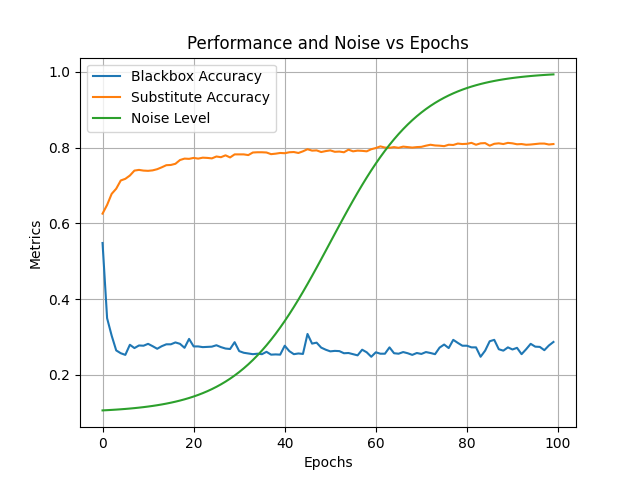
\includegraphics[width=0.8\linewidth]{images/graph_100_epochs.png}
        \caption{\emph{Andamento delle metriche su 100 epoche di addestramento}}
        \label{fig:graph_100_epochs}
\end{figure}

\subsection{Risultati Esperimento 2}
Di seguito vengono analizzati i risultati del secondo esperimento condotto con il modello GAN.
\subsubsection{Risultati Blackbox}
I risultati mostrano che il modello Blackbox è fortemente influenzato dall'aumento del livello di rumore generato. Mentre all'inizio dell'addestramento le prestazioni sono moderate, con un'accuratezza intorno al 60\%, queste subiscono un degrado significativo con il crescere del rumore. Nelle fasi finali dell'addestramento, quando il livello di rumore raggiunge valori elevati, il modello diventa incapace di fare previsioni significative, con metriche che si stabilizzano su livelli molto bassi. Questo comportamento evidenzia la vulnerabilità del Blackbox a perturbazioni avversarie.
\subsubsection{Risultati Substitute Detector}
Il Substitute Detector, al contrario, si dimostra molto più resiliente al rumore. Fin dalle prime fasi dell'addestramento, le sue prestazioni sono superiori rispetto al Blackbox, e continuano a migliorare progressivamente. Anche in presenza di un rumore significativo, il Substitute mantiene un'elevata accuratezza e robustezza, confermandosi una soluzione più adatta in contesti avversari.
\subsubsection{Impatto del livello di rumore}
L'impatto del rumore è evidente, poiché il suo progressivo aumento compromette rapidamente le prestazioni del Blackbox. Il GAN genera perturbazioni sempre più efficaci, che rendono il modello Blackbox incapace di adattarsi. Tuttavia, il Substitute Detector dimostra di essere meno sensibile a questo fenomeno, mantenendo alte prestazioni anche in presenza di livelli di rumore molto elevati.
\subsubsection{Conclusioni}
In conclusione, l'esperimento evidenzia la vulnerabilità del modello Blackbox e l'efficacia del Substitute Detector nel mantenere alte prestazioni nonostante l'incremento del rumore. Il GAN si conferma una strategia efficace nel generare perturbazioni avversarie, ma i risultati suggeriscono che modelli più robusti, come il Substitute, possono rappresentare una valida difesa contro questo tipo di attacchi.
\begin{figure}[ht]
    \centering
        \centering
        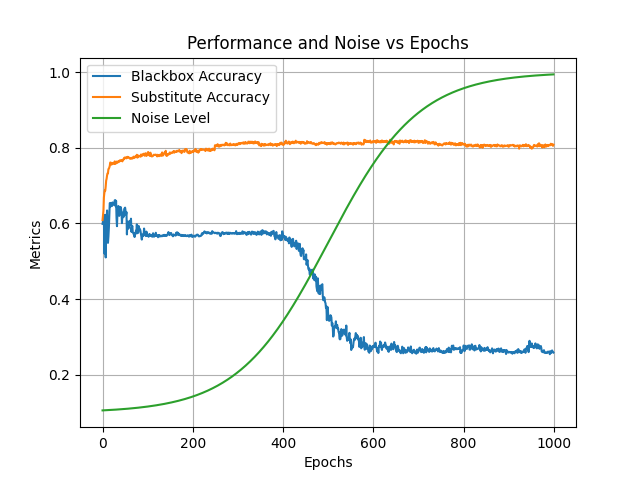
\includegraphics[width=0.8\linewidth]{images/graph_1000_epochs_64batch.png}
        \caption{\emph{Andamento delle metriche su 1000 epoche con batch size 64}}
        \label{fig:graph_1000_epochs_batch_64}
\end{figure}

\subsection{Risultati Esperimento 3}
Di seguito viene presentata un'analisi dei risultati del terzo esperimento condotto con il modello GAN.
\subsubsection{Risultati Blackbox}
Si può notare come, a differenza dell'esperimento precedente, il modello Blackbox (lina blu) parta con un'accuratezza inferiore al 40\%, che diminuisce drasticamente nelle prime epoche di addestramento, fino a raggiungere un livello inferiore al 25\%. Tuttavia, nonostante l'aumento del rumore nelle ultime epoche finali, si può notare come il modello mantenga una certa capacità di classificazione, seppur molto limitata.

\subsubsection{Risultati Substitute Detector}
L'accuratezza del discriminatore (linea arancione) si stabilizza rapidamente oltre l'80\%, mostrando una capacità costante di classificare correttamente sia le immagini reali sia quelle generate. Questo risultato evidenzia che il discriminatore riesce ad adattarsi efficacemente alle immagini alterate create dal generatore.

\subsubsection{Impatto del livello di rumore}
Il livello di rumore (linea verde) aumenta in modo progressivo durante le epoche, seguendo un andamento sigmoideo. Questo incremento controllato del rumore contribuisce sia alla riduzione dell'accuratezza del Blackbox sia al mantenimento delle prestazioni del discriminatore. La sinergia tra questi elementi è cruciale per il successo dell'addestramento.

\subsubsection{Conclusioni}
Il grafico mostra che il framework proposto riesce a ottenere un compromesso efficace: il generatore inganna il modello Blackbox riducendone l'accuratezza, mentre il discriminatore mantiene prestazioni elevate. L'aumento progressivo del rumore è un fattore determinante nel raggiungimento di questi risultati, dimostrando l'importanza della strategia di addestramento adottata.
\begin{figure}[ht]
    \centering
        \centering
        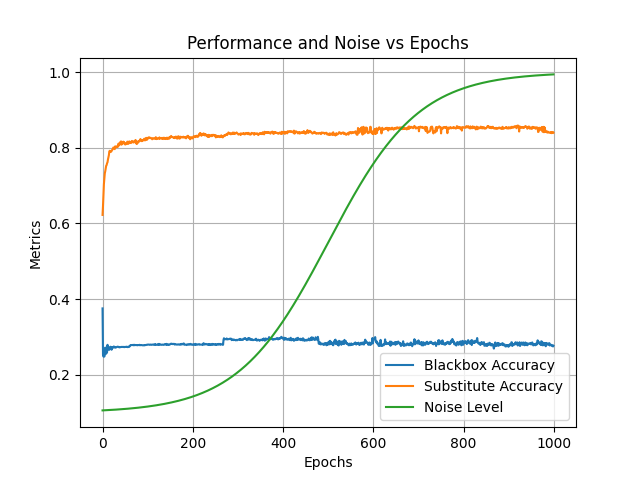
\includegraphics[width=0.8\linewidth]{images/graph_1000_epochs_32batch.png}
        \caption{\emph{Andamento delle metriche su 1000 epoche con batch size 32}}
        \label{fig:graph_1000_epochs_batch_32}
\end{figure}

\subsection{Applicazione Grad-CAM}
La Grad-CAM (Gradient-weighted Class Activation Mapping)\cite{site:gradcam} è stata utilizzata in questo studio come strumento fondamentale per interpretare il comportamento dei modelli in presenza di rumore crescente. L'obiettivo principale dell'adozione della Grad-CAM è stato quello di ottenere una visualizzazione chiara delle aree di interesse del modello durante la classificazione, specialmente quando il livello di rumore incrementale introdotto dal generatore potrebbe alterare le decisioni del modello.
\subsubsection{Interpretabilità del modello}
La Grad-CAM consente di evidenziare le regioni dell'immagine che contribuiscono maggiormente alla decisione del modello. Questa capacità di visualizzazione aiuta a comprendere se il modello si concentra su caratteristiche rilevanti o viene invece distratto da perturbazioni indotte dal rumore.
\subsubsection{Valutazione dell'impatto del rumore}
L'adozione della Grad-CAM permette di analizzare come l'incremento del rumore influenza le regioni di attenzione del modello. Come mostrato nelle immagini, al crescere del rumore, le attivazioni diventano sempre più distribuite in maniera casuale, indicando che il modello potrebbe perdere la capacità di concentrarsi sulle caratteristiche salienti dell'immagine.

\begin{figure}[ht]
    \centering
    \begin{minipage}{0.45\textwidth}
        \centering
        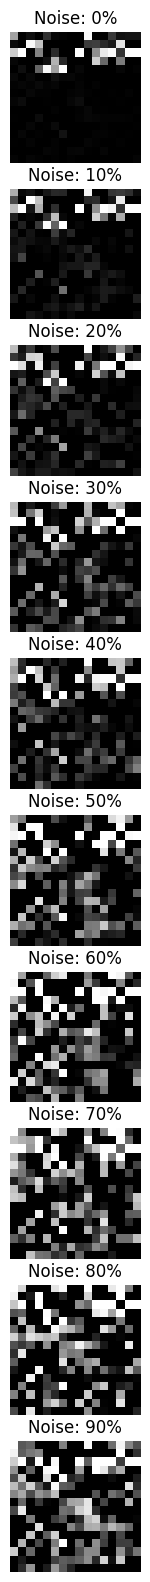
\includegraphics[width=0.31\linewidth]{images/vertical_noise_grid_100.png}
        \label{fig:rumore_scala_grigi}
    \end{minipage}\hfill
    \begin{minipage}{0.45\textwidth}
        \centering
        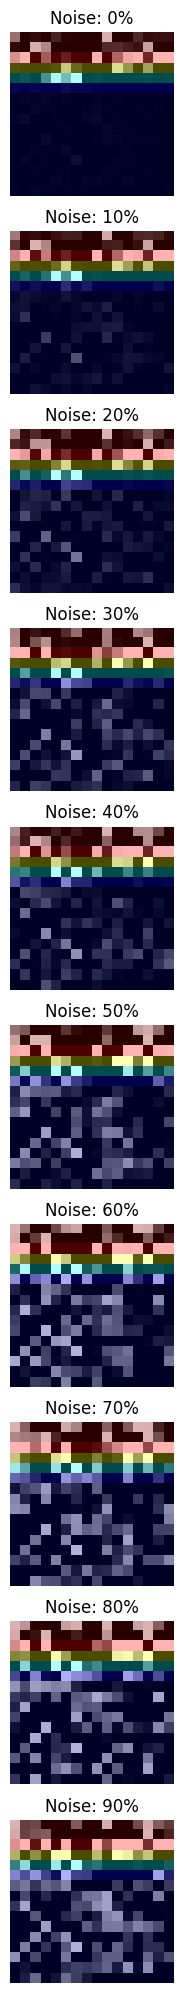
\includegraphics[width=0.3\linewidth]{images/vertical_gradcam_noise_grid_100.png}
        \label{fig:grad_cam}
    \end{minipage}
    \caption{\emph{Rumore generato dal generatore (a sinistra) e Grad-CAM applicato al modello sostitutivo (a destra) per un malware di famiglia Trojan}}
\end{figure}
~\\
